%%%%%%%%%%%%%%%%%%%%%%%%%%%%%%%%%%%%%%%%%%%
\section{Numerical Experiments}\label{sec_numexp}
%%%%%%%%%%%%%%%%%%%%%%%%%%%%%%%%%%%%%%%%%%%
In this section, we highlight our results by examining the numerical behavior of the iterates and derivatives for an application. 
All the experiments were carry out using Matlab software (\cite{matlab22}). 

We consider that we want solve the following linear inverse problem 
\begin{equation}\label{eq:inv-probl}\tag{$\calP_{\mathrm{inv}}$}
\begin {cases}
\text{Recover a real vector or signal $\avx(\theta)\in \bbR^n,$  from }\\
y(\theta)= A\avx(\theta)\in \bbR^m \qwhereq \avx(\theta)=\frac{1}{2}\tilde{x}\theta^2, 
\end{cases}
\end{equation}
where we have $A\in \bbR^{m\times n}$ is the measurements matrix whose rows $(a_r)_{r\in[m]}$ are the measurements vectors.  Our parameter   $\theta\in\bbR$  can be seen as a scaling coefficient of the fixed signal  $\tilde{x}\in\bbR^n$ which is also a fixed vector.

\subsection{Solving using Least-squares or linear regression}\label{sec:least-square}
To solve \eqref{eq:inv-probl}, we consider the following parametric optimization problem  
\begin{equation}\label{eq:param-ls}
\forall \theta\in\bbR, \quad \min_{x\in\bbR^n}f(x,\theta)=\frac{1}{2}\normm{y(\theta)-Ax}^2.
\end{equation}
 For all $ x\in\bbR^n, \theta\in\bbR$, we have 
\begin{align}\label{eq:derivative}
\nabla_x f(x,\theta)=-\transp{A}\Ppa{y(\theta)-Ax},\quad\nabla^2_x f(x,\theta)=\transp{A}A,\qandq\nabla^2_{x\theta} f(x,\theta)=-\pa{\transp{A}A}\tilde{x}\theta.
\end{align}
From \eqref{eq:derivative}, we have that $\forall \theta \in \Theta$ 
\begin{align}
\normm{\nabla_x f(x,\theta)-\nabla_x f(z,\theta)} \leq \normm{A} \normm{x-y},
\end{align}
thus the Lipschitz-coefficient is given by $L=\normm{A}.$
 
We recall that our goal is to solve \ref{eq:param-ls} using the inertial scheme Algorithm~\ref{eq:inertial-methods} and then differential through the latter. Given any smooth function of $\theta$ as an initial point: $\forall \theta\in \bbR, \xo(\theta)\in\bbR^m$, we define $X_0(\theta)=\begin{pmatrix} \xo(\theta)\\ \xo(\theta)\end{pmatrix}$ then the automatic differentiation produces the following sequence:
\begin{multline}
 \forall k\in\bbN, \quad  \hspace{-0.2cm} \partial_{\theta}X_{k+1}(\theta)= \begin{pmatrix} (1+\ak)\Id-\gak(1+\bk)\transp{A}A &-\ak\Id+\gak\bk\transp{A}A \\
		 \Id  & 0\end{pmatrix}\partial_{\theta}X_k(\theta)\\+\begin{pmatrix} \gak\pa{\transp{A}A}\tilde{x}\theta  \\  
		0\end{pmatrix}.
\end{multline}
Thanks to  the explicit formula \eqref{eq:expli-form}, we get 
  \begin{equation}
 \hspace{-0.8cm}\partial_{\theta}X^{\star}\pa{\theta}=\begin{pmatrix} -a\Id+\gamma(1+b)\transp{A}A &a\Id-\gamma b\transp{A}A \\ -\Id  & 
		\Id\end{pmatrix}^{-1}\hspace{-0.2cm}\begin{pmatrix} \gamma\pa{\transp{A}A}\tilde{x}\theta  \\  
		0\end{pmatrix}.
\end{equation}
\begin{remark} Although this Ordinary least-square case looks very basic, it is important  and as highlights, the computations are done handily so that we can observe the behaviour of our  differentiation procedure throughout.   
\end{remark}
\vspace{-0.8cm}
\paragraph{Experience setup} 
In our numerical simulations, we suppose that $\forall r \in [m],  a_r \stackrel{\footnotesize{\text{\iid}}}{\sim}\calN(0,\Id)$ and the Lipschitz coefficient of the gradient $L\approx\sqrt{m}$. Moreover, we choose for simplicity that  $\xo\in\bbR^n,$ a constant function of $\theta$ which implies that $\partial_{\theta}\xo(\theta)=0$. For each simulation, we run the inertial scheme for $400$ iterations and  we compare  the results with the solution $\xsol(\theta)$ and his derivatives $\partial_{\theta}\xsol(\theta)$. Finally,  we select the parameters of our algorithm  to get two different scenario: 
\begin{itemize}
\item \textbf{Case 1:} $\gak\equiv\frac{1}{L-2/k}, \ak=\bk=\frac{k-1}{k+20}.$ We easily get that $a=b=1$ and $\gamma=1/L.$
\item \textbf{Case 2:} $\gak\equiv\frac{1}{L-2/k}, \ak=\bk=0,$ with  $a=b=0$ and $\gamma=1/L.$
\end{itemize}
\begin{figure}[htbp]
\centering
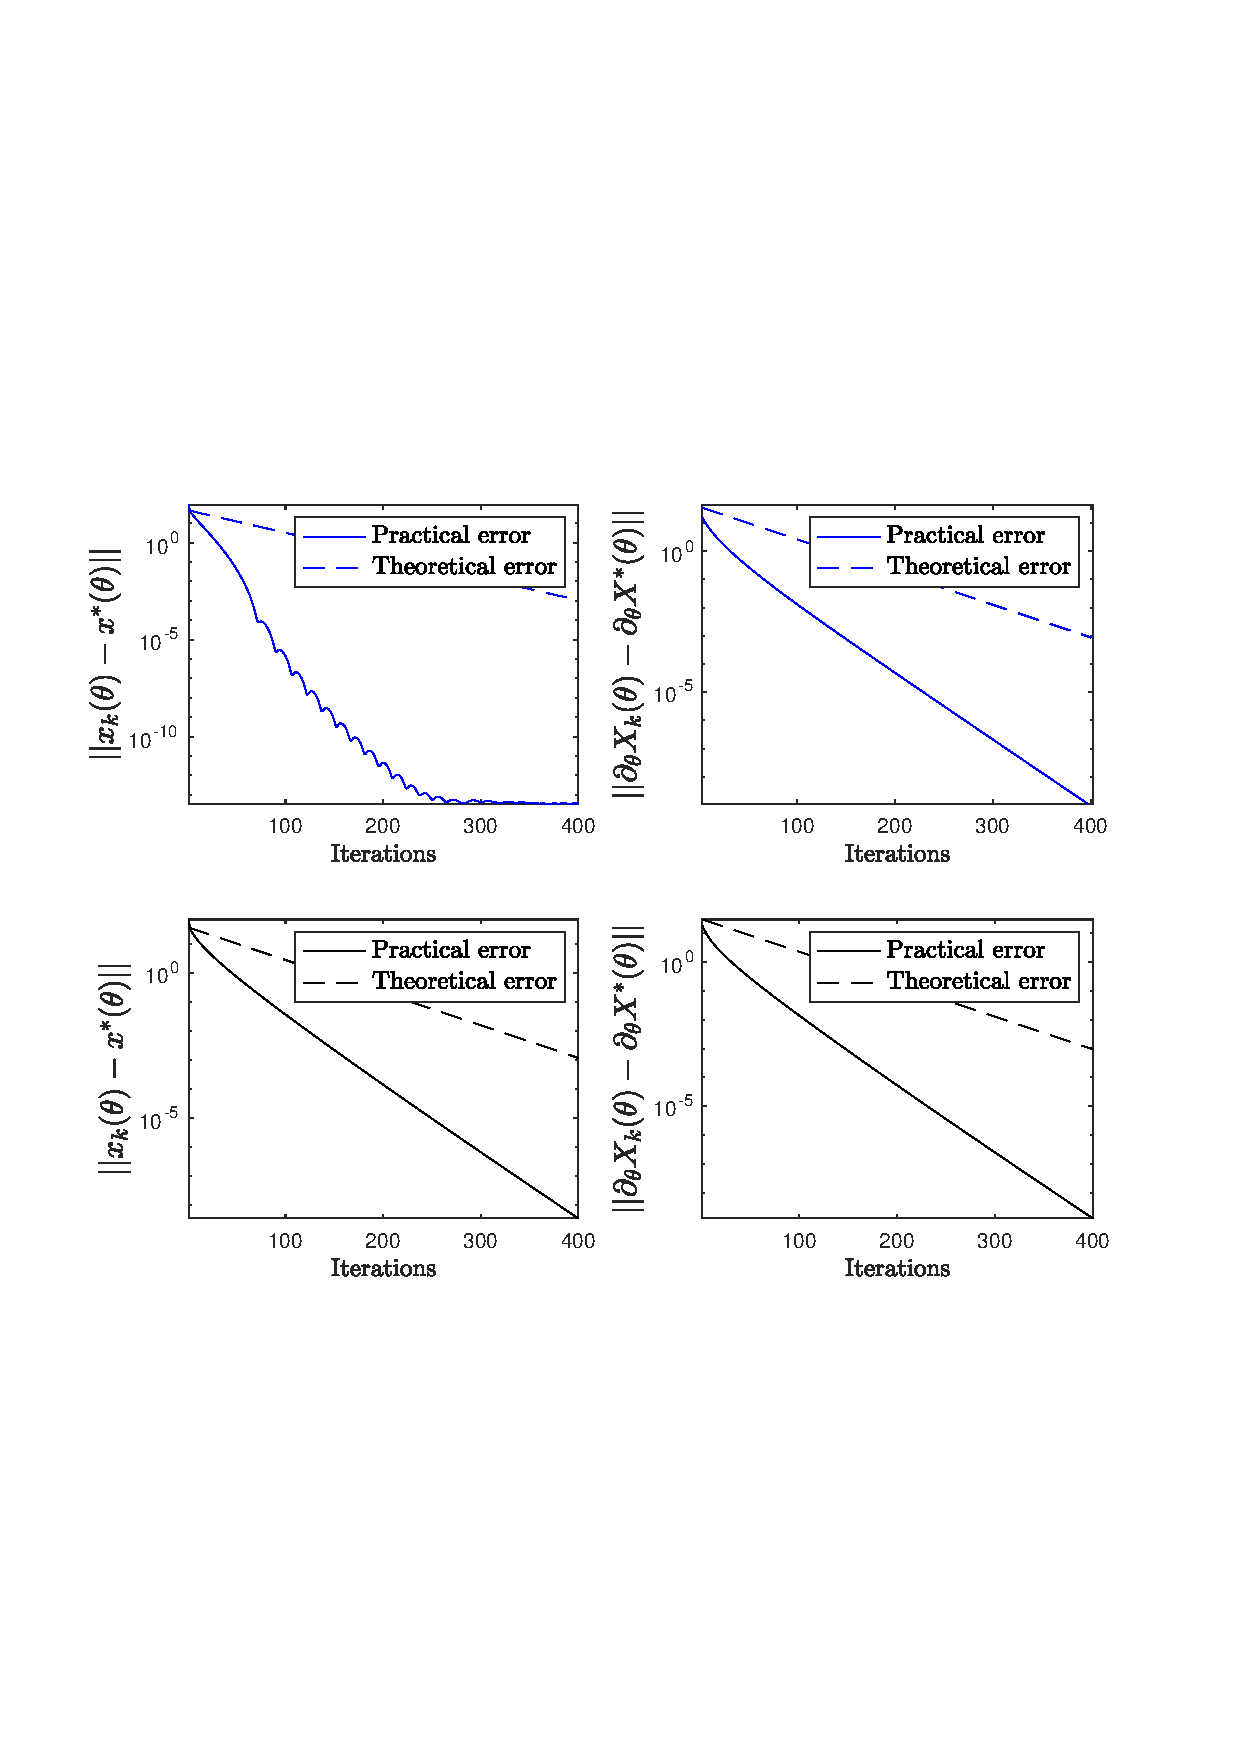
\includegraphics[trim={0cm 8.5cm 0cm 8.5cm},clip,width=1\textwidth]{figures/ls.pdf}
 \caption{Automatic differentiation of the inertial methods (Case 1=inertial method) and (Case 2=  Gradient  descent).}
\label{fig: linea-inv-vstep}
\end{figure} 

\paragraph{Observations }  In Figure~\ref{fig: linea-inv-vstep}, we  displayed the result of our numerical experiments for solving the problem \eqref{eq:inv-probl}  with the least-square formulation \eqref{eq:param-ls}. The first line in blue is the result when we use a standard inertial method. On the left hand side, we have the  error of the of the inertial schemes with respect to the number of iterations and in dashed line we have the Theoretical error which is of course not optimistic. We can  observe with the experiments oscillations which characterize inertial methods. On the right hand side, the error of the differentiation methods with respect to the number of iterations. In dashed line, the theoretical linear convergence without the error term and in plain line the observed error.  As predicted by Theorem~\ref{thm:conv-rat-der}, the linear convergence does not occur from the start as described by many automatic differentiation daily users. We have a small regime without the linear convergence. In this regime, the error term is large which impact the convergence of the differentiation scheme.  We can see that the error is not linear. But after a few iterations the differentiation procedure enters a linear convergence regime. And  this is what we have highlighted in our Theorem~\ref{thm:conv-rat-der}. Moreover, as predicted in Remark~\ref{rmk:inert-deriv}, after differentiation they are no more oscillations, we have a linear convergence after few iterations. On the second scenario, we solved the problem using the gradient descent and plotted the results in black. We  can observe in contrast to the previous case that we  do not have oscillations which also describe this scheme. We have made the same experiments, and on the left hand side, after few iterations, the sequence enters a linear convergence rate. On the right side, the differentiation of the gradient descent show the same behaviour as the  sequence generated by the gradient descent. Theses numerical experiments confirm all our theoretical results.  
%\subsection{Logistic regression }\label{sec:loreg}
%In this subsection, we aim to solve the inverse problem using logistic regression. Thus, we consider  the following objective function
%\begin{equation}\label{eq:param-loreg}
%\forall \theta\in\bbR, \quad \min_{x\in\bbR^n}f(x,\theta)=\sum_{i=1}^m\log\Ppa{e^{\pa{Ax}_i}+1}-\Ppa{y(\theta)}_i \pa{Ax}_i. 
%\end{equation}
%By setting $u\eqdef\Ppa{1,1,\cdots,1}$, we can rewrite the objective function in \eqref{eq:param-loreg} as follow 
%\begin{equation}\label{eq:pam-loreg}
%\forall \theta\in\bbR, \quad f(x,\theta)= \pscal{\log\Ppa{e^{Ax}+u};u}_{\bbR^m} - \pscal{y(\theta);Ax}_{\bbR^m}.
%\end{equation}
 %Let us mention that we suppose that the one-dimensional functions (logarithm and exponential) act on vectors component-wise such as binary operations. Under this, the gradient of this function with respect  to the first variable is given by
 %\[
 %\nabla_x f(x,\theta)=-\transp{A}y(\theta)+\transp{A}\Ppa{\frac{e^{Ax}}{e^{Ax}+u}},
 %\]
 %thus the Lipschitz coefficient of the gradient $L=\normm{A}\frac{\sqrt{m}}{4}e^{\normm{A}}\approx \frac{me^{\sqrt{m}}}{4}.$
 
 
 %The second order derivatives with respect to the first variable
 %\[
 %\nabla_x^2 f(x,\theta)=\transp{A}\mathrm{diag}\Ppa{\frac{e^{Ax}}{e^{Ax}+u}}A-\transp{A}e^{Ax}\transp{\Ppa{\frac{e^{Ax}}{\Ppa{e^{Ax}+u}^2}}}A,
 %\]
 %and the second order derivative with respect to the second variable is given by
%\[
%\nabla_{x\theta}^2f(x,\theta)=-\transp{A}\partial_{\theta}y(\theta).
%\]
%\subsection{Solving using the log-exponential}\label{sec:logexp}
%Let us start by briefly introduce what is called the log-exponential function  \ie 
%\begin{equation}
%\forall x \in \bbR^m,\quad  \logexp(x)\eqdef \log\BPa{e^{x_1}+\cdots+e^{x_m}}.
%\end{equation} 
%According to \cite[Example~2.16]{rockafellar_variational_1998}, the log-exponential function is only a convex function. However, in the context of solving \eqref{eq:inv-probl}, we consider  the following parametric optimization problem  
%\begin{equation}\label{eq:param-logexp}
%\forall \theta\in\bbR, \quad \min_{x\in\bbR^n}f(x,\theta)=\frac{1}{2}\BPa{\logexp\Ppa{y(\theta)-Ax}}^2,
%\end{equation}
%To simplify the notations, we denote by $\sigma(y)\eqdef\sum_{j=1}^me^{y_j}, \forall y\in \bbR^m$. We rewrite \eqref{eq:param-logexp} as
%\[
%\forall \theta\in\bbR,\quad f(x,\theta)=\frac{1}{2}\BPa{\log\pa{\sigma\Ppa{y(\theta)-Ax}}}^2.
%\]
%We have that,  for all $ x\in\bbR^n, \theta\in\bbR$  we have that the gradient  of $f$ is given
%\begin{equation}\label{eq:gradient-formula}
%\nabla_x f(x,\theta)=\frac{-\logexp\Ppa{y(\theta)-Ax}}{\sigma\Ppa{y(\theta)-Ax}}\transp{A}\nabla\sigma\Ppa{y(\theta)-Ax}.
%\end{equation}
 %The second order derivatives of interest are respectively
%\begin{multline}\label{eq:hes_xx}
%\nabla^2_xf(x,\theta)=\frac{\logexp\Ppa{y(\theta)-Ax}-1}{\sigma\Ppa{y(\theta)-Ax}^2}\transp{\BPa{\nabla\sigma\Ppa{y(\theta)-Ax}A}}\nabla\sigma\pa{y(\theta)-Ax}A\\-\frac{\logexp\Ppa{y(\theta)-Ax}}{\sigma\pa{y(\theta)-Ax}}\transp{A}\BPa{\diag{\nabla\sigma\pa{y(\theta)-Ax}}}A,
%\end{multline}
 %and 
%\begin{multline}\label{eq:hes_xt}
%\nabla^2_{x\theta}f(x,\theta)=\frac{\logexp\Ppa{y(\theta)-Ax}-1}{\sigma\Ppa{y(\theta)-Ax}^2}\transp{\BPa{\nabla\sigma\Ppa{y(\theta)-Ax}A}}\nabla\sigma\pa{y(\theta)-Ax}\tilde{x}\theta\\-\frac{\logexp\Ppa{y(\theta)-Ax}}{\sigma\pa{y(\theta)-Ax}}\transp{A}\BPa{\diag{\nabla\sigma\pa{y(\theta)-Ax}}}\tilde{x}\theta.
%\end{multline}
%where 
%$
%\quad\nabla\sigma(y)=\begin{pmatrix}e^{y_1}\\\vdots\\e^{y_m}\end{pmatrix}.$
%As previously, given any smooth function of $\theta$ as an initial point:\\
 %$\forall \theta\in \bbR, \xo(\theta)\in\bbR^m$, we define $X_0(\theta)=\begin{pmatrix} \xo(\theta)\\ \xo(\theta)\end{pmatrix}$ then the automatic differentiation produces the following sequence: $ \forall k\in\bbN, $
%\[
%\ybk(\xk,\xkm)=\xk\pa{\theta}+\bk\pa{\xk\pa{\theta}-\xkm\pa{\theta}},
%\]
%\begin{multline}
% \hspace{-0.2cm} \partial_{\theta}X_{k+1}(\theta)= \begin{pmatrix} (1+\ak)\Id-\gak(1+\bk)\nabla^2_xf\pa{\ybk\pa{\xk,\xkm},\theta} &-\ak\Id+\gak\bk\nabla^2_xf\pa{\ybk\pa{\xk,\xkm},\theta} \\
%		 \Id  & 0\end{pmatrix}\\\partial_{\theta}X_k(\theta)+\begin{pmatrix}-\gak\nabla_{x\theta}^2f\pa{\ybk\pa{\xk,\xkm},\theta} \\  
%		0\end{pmatrix}.
%\end{multline}
%Where the different formulas are in \eqref{eq:hes_xx} and \eqref{eq:hes_xt}. Finally, we have
 %\begin{equation}
 %\hspace{-0.8cm}\partial_{\theta}X^{\star}\pa{\theta}=\begin{pmatrix} -a\Id+\gamma(1+b)\nabla_x^2f(\xsol(\theta),\theta) &a\Id-\gamma b\nabla_x^2f(\xsol\pa{\theta},\theta) \\ -\Id  & 
%		\Id\end{pmatrix}^{-1}\hspace{-0.2cm}\begin{pmatrix} -\gamma\nabla_{x\theta}^2f(\xsol,\theta)  \\  
%		0\end{pmatrix}.
%\end{equation}

%\paragraph{Observations }   We have re-introduced the log-exponential function in view to solve linear inverse problem as an alternative to logistic regression most commonly used in the learning literature. 
%In this work, we wish to differentiate through  the inertial methods to solve this problem as the previous  example and  without any mathematical background and we encounter some  difficulties.  Regarding differentiation,  we do not have strong convexity or unicity of the minimizer. Therefore, our theoretical results are not directly applicable. However, we observe that  for any $\theta \in \Theta$ at $\xbar(\theta)$
%\begin{align*}
%\nabla f(\xbar(\theta))=0,\qandq  \nabla_x^2 f(\xbar(\theta),\theta)=-\frac{e}{m}\transp{A}A\preceq0.
%\end{align*}
%This  suggests that $\xbar(\theta)$ is a particular critical point of of $f(x,\theta)$. We will investigate  the properties of this function for solving linear inverse problem and his differentiation in a future work.   





















